\section{Word Classes: Validation and Frequency Bins}
\label{app:wordclass}

\subsection{Do the DLT classes index processing difficulty?}
\label{app:wordclass-dlt}

\paragraph{Parsing.} DLT costs (Section~\ref{sec:design-dlt}) are computed from a parse of the full text of each dataset with its punctuation, so that the parser sees sentence boundaries; for GECO the words are taken with their punctuation from the reading data. The Podcast transcript is punctuated on 5 of its 5,136 words, so it is first segmented into sentences: a sentence starts at a word that follows sentence-final punctuation, at a capitalized word that also occurs in lower case elsewhere in the transcript, or at an always-capitalized word (a name or \textit{I}) preceded by a pause longer than 350\,ms. This gives about 410 sentences of 12.5 words on average; parsed as unsegmented text, the transcript yields run-on ``sentences'' of about 50 words and dependencies that cross sentence boundaries.

\begin{figure}[h]
\centering
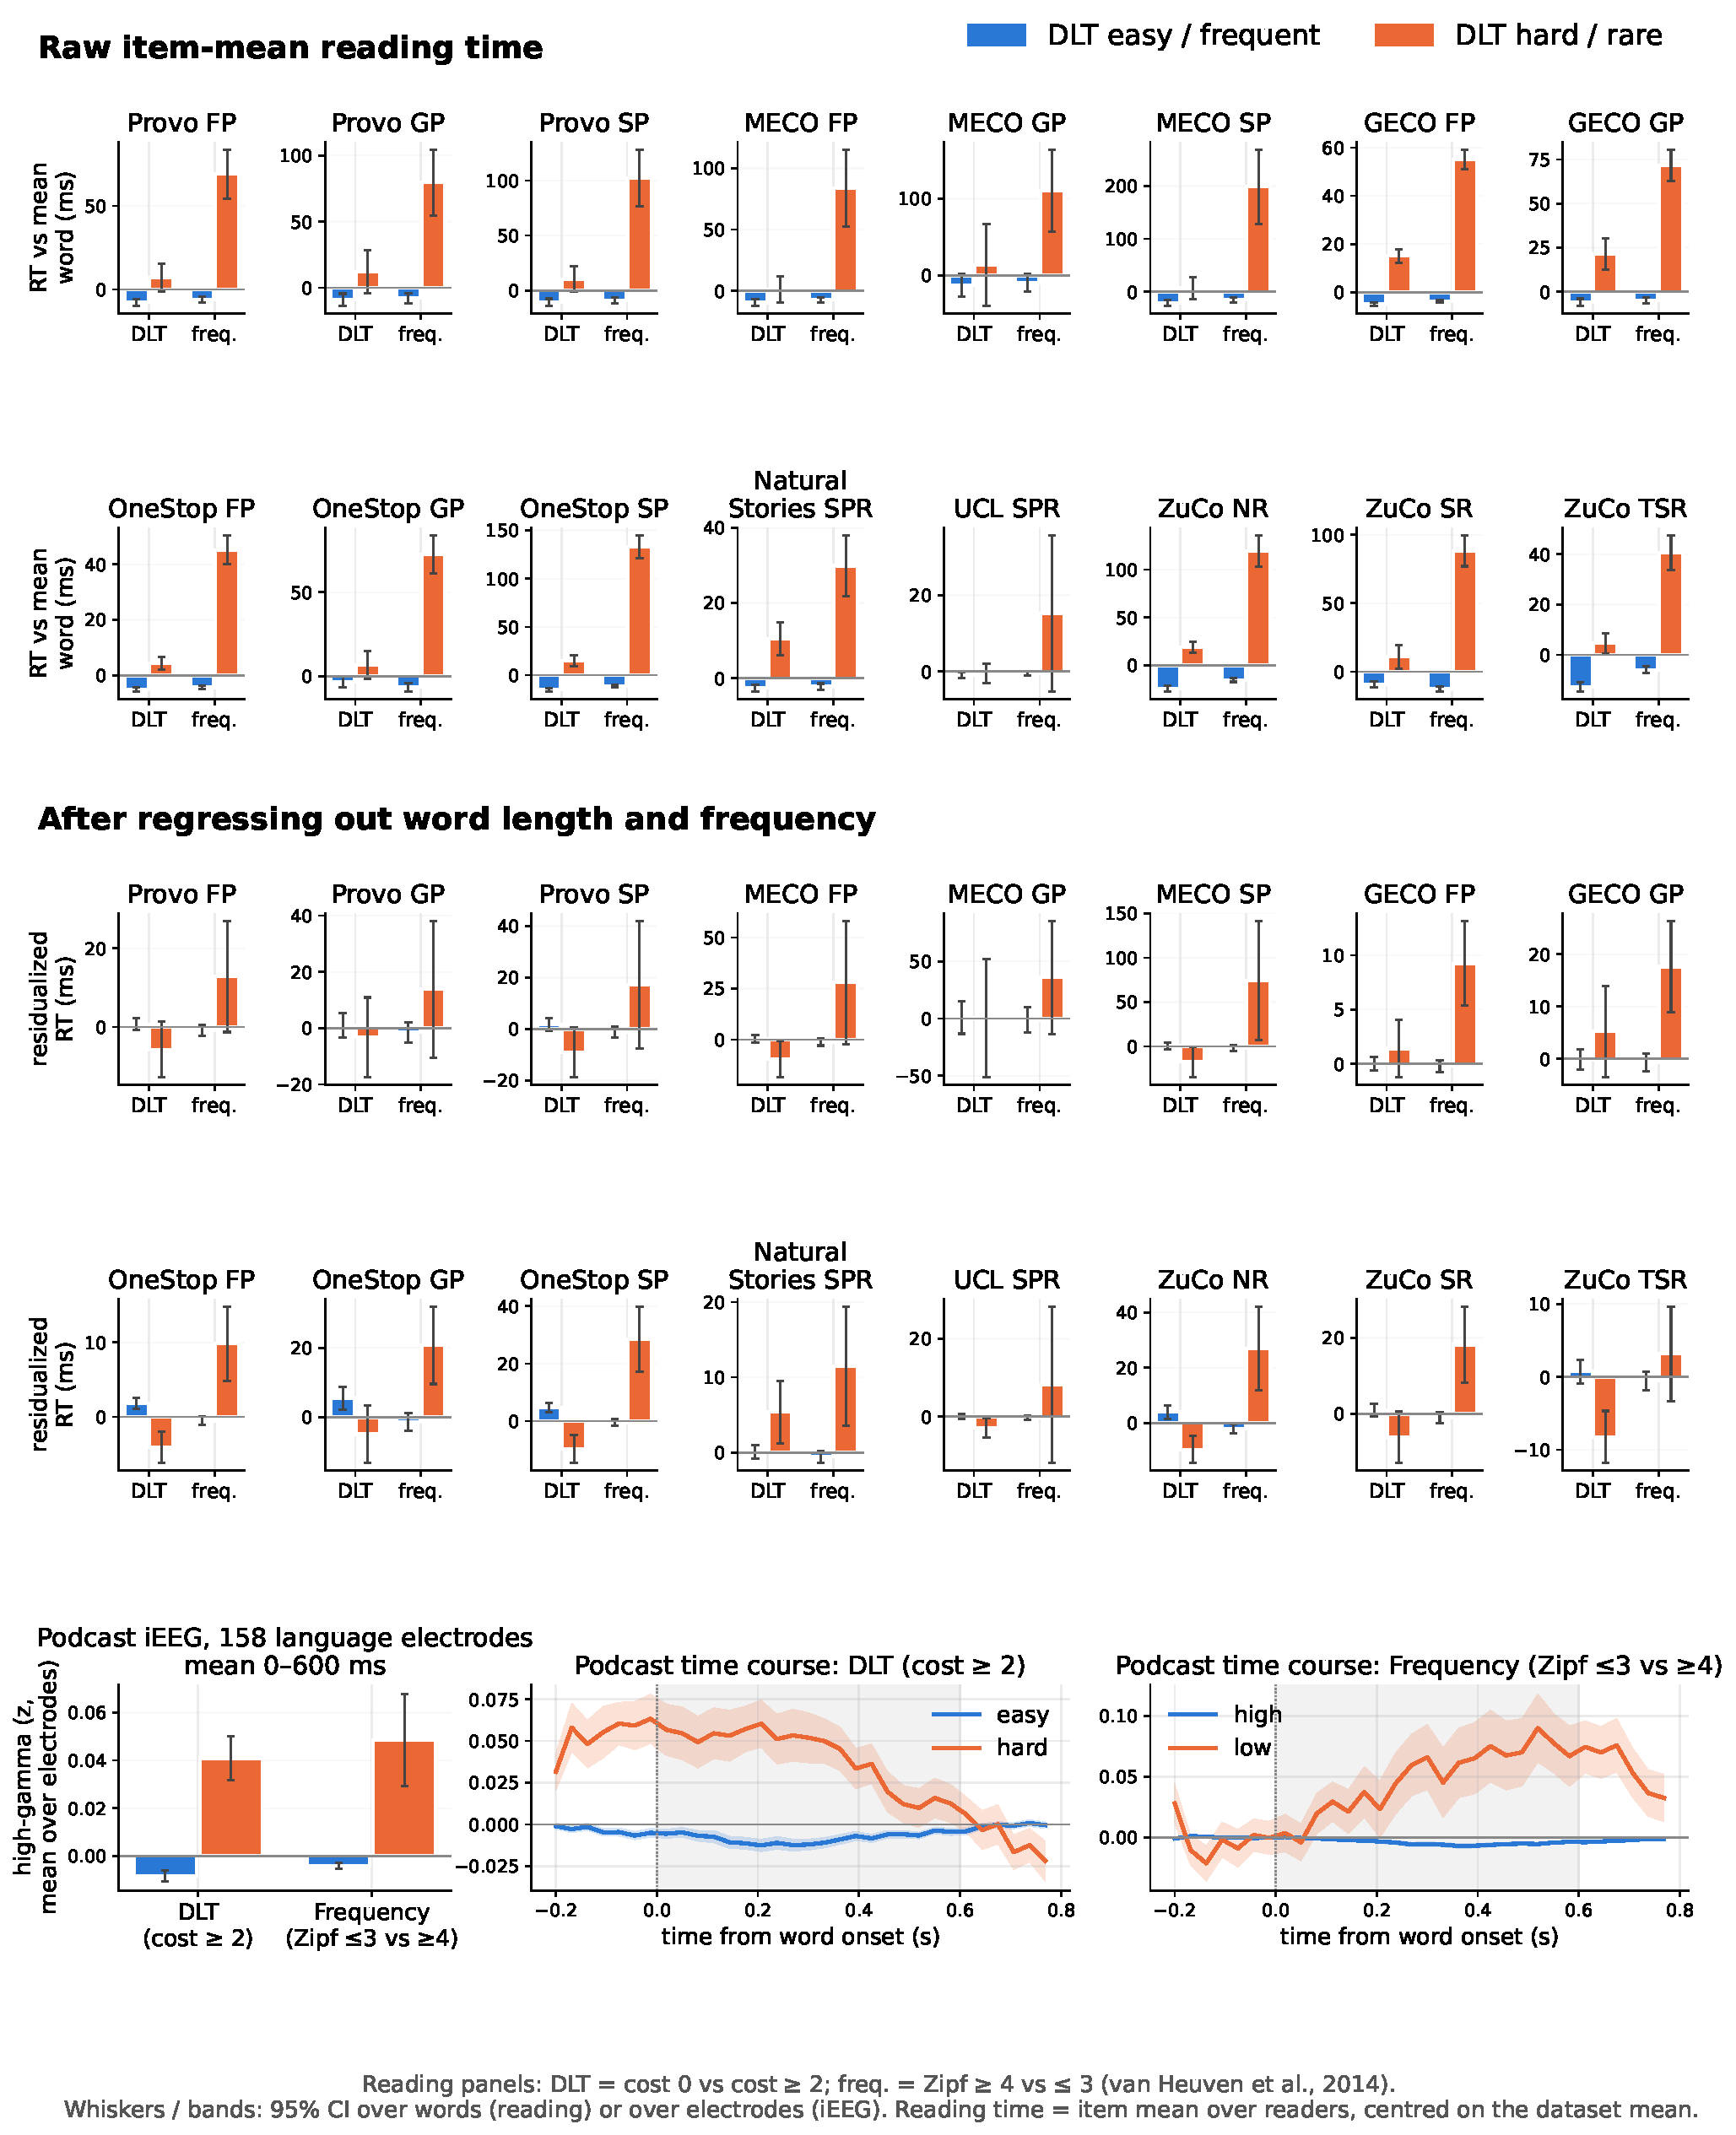
\includegraphics[width=\linewidth]{figures/appendix_wordclass_human.pdf}
\caption{Human responses to the word classes. Reading panels: item-mean reading time over participants (the response of the RDM regression), relative to the mean word (top two rows) and after an ordinary least-squares regression on word length (letters) and Zipf frequency within the measure (bottom two rows), for DLT-easy (cost 0) and DLT-hard (cost $\geq 2$) words and for frequent and rare words (Zipf $\geq 4$ vs.\ $\leq 3$, the bins of Appendix~\ref{app:wordclass-freq}). Rare words stay slower after the linear frequency regression because reading time rises faster than linearly at low frequency. Podcast: high-gamma activity of the 158 language electrodes, z-scored per electrode and lag, mean over 0--600\,ms and time courses. Whiskers and bands: 95\% confidence intervals over words (reading) or electrodes (ECoG).}
\label{fig:wordclass-human}
\end{figure}

\paragraph{Reading times.} Hard words are read more slowly than easy words in nearly every measure (Figure~\ref{fig:wordclass-human}), but they are also longer and rarer (by 1.2--1.7 Zipf units). After regressing out word length and frequency, the difference remains only in Natural Stories self-paced reading ($+5.3$\,ms, 95\% CI $[1.1, 9.5]$; 603 hard and 6,732 easy words). It is not reliable in GECO (first pass $+1.4$\,ms $[-1.3, 4.1]$; go-past $+5.3$\,ms $[-3.6, 14.2]$), and absent or reversed in the other measures, where hard words are read as fast as or faster than words of the same length and frequency (e.g.\ OneStop scan-path time $-14.3$\,ms, ZuCo normal reading $-13.5$\,ms, MECO scan-path time $-17.9$\,ms; Provo and MECO have only 95--116 hard words). Rare words, by contrast, are read more slowly than frequent words of the same length in every measure (Appendix~\ref{app:wordclass-freq}).

\begin{figure}[h]
\centering
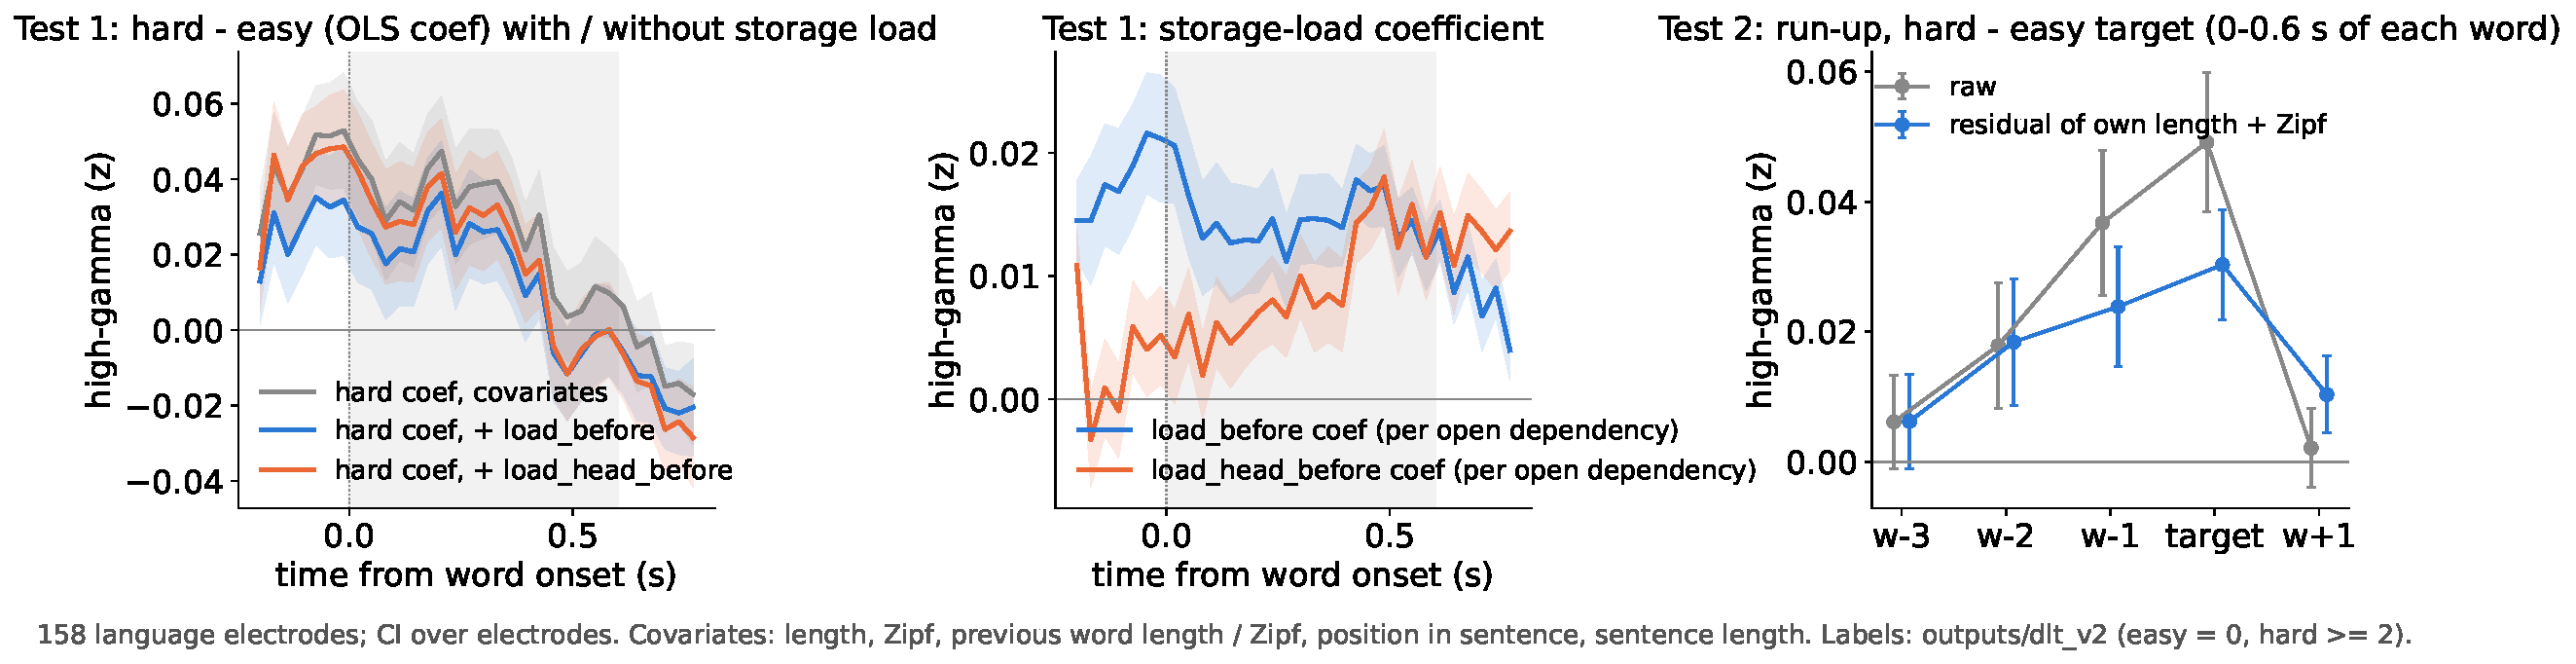
\includegraphics[width=\linewidth]{figures/appendix_podcast_dlt_runup.pdf}
\caption{Podcast high-gamma activity around DLT-hard words (158 language electrodes; 95\% confidence intervals over electrodes). Left: hard $-$ easy coefficient of an ordinary least-squares regression per electrode and lag with word length and frequency, previous-word length and frequency, position in the sentence and sentence length as covariates, without and with the number of open dependencies. Middle: coefficient of the number of open dependencies. Right: activity (0--600\,ms) of the words preceding and following hard and easy words, after regressing out each word's own length and frequency.}
\label{fig:podcast-runup}
\end{figure}

\paragraph{Podcast.} Activity over 0--600\,ms is higher for hard than for easy words ($+0.049$\,z; 244 hard and 3,332 easy words), but the difference is already present before word onset and remains when length, frequency, the previous word and the position in the sentence are controlled. It builds up over the words that lead to a hard word and falls after it (Figure~\ref{fig:podcast-runup}, right): $+0.006$\,z three words before (not reliable), $+0.018$ two words before, $+0.024$ one word before, $+0.030$ on the hard word and $+0.010$ on the next word. A response of the preceding word overlapping the hard word's window would raise only the immediately preceding word, and the word two positions back starts about 0.6\,s before the hard word. The rise tracks the number of dependencies that are open when a word starts (Figure~\ref{fig:podcast-runup}, middle): each open dependency adds $+0.015$\,z ($\pm0.003$), and this count absorbs about 45\% of the hard-word difference, which remains reliable ($+0.016$\,z). We read the Podcast effect as activity sustained while a dependency is held open and released when it is completed, consistent with the build-up of language-network activity over a sentence \citep{fedorenko2016neural}, rather than as a response evoked by the hard word. The count of open dependencies comes from the same parse as the DLT classes, so the run-up, which uses only each word's own activity, is the more independent evidence.

\paragraph{Scale of the bins.} Both bins are divided by the all-pairs reference, so a bin's score is its share of the dataset's reliable signal, and the any-hard bin carries more of it (median model .073 of the reference in Natural Stories, against .013 on easy--easy pairs). A constraint that raised scores by the same proportion in both bins would therefore get a larger coefficient on any-hard pairs, as size and perplexity do. On the logarithm of the score, coefficients are proportional changes and this difference of scale drops out. On this outcome (fitted by ordinary least squares with family-clustered standard errors), neither constraint differs between bins (memory $-.038$, $p=.75$; data $-.096$, $p=.19$; all behavioral scores are positive, so no model is dropped). The larger constraint coefficients on any-hard pairs in Table~\ref{tab:summary}, whose bin differences are themselves not reliable, are thus larger in units of the human signal, not in relative terms.

\subsection{Frequent and rare words}
\label{app:wordclass-freq}


\paragraph{Bins.} A word is \emph{frequent} if its Zipf frequency (the value of the frequency confound RDM) is at least 4 and \emph{rare} if it is at most 3, the thresholds that \citet{vanheuven2014subtlex} give for high- and low-frequency words on the Zipf scale; words between 3 and 4 are left out. We keep the datasets with at least 100 rare words: the 9 measures of GECO, OneStop, Natural Stories and ZuCo (275 rare words in Natural Stories, 328--1{,}044 in the others) and Podcast (126 rare words); UCL (7 rare words), Provo (47) and MECO (51) are excluded. Unlike the DLT classes, these bins index processing difficulty in every dataset used. After regressing out word length, rare words are read more slowly than frequent ones in all 9 measures, by 15 to 99\,ms (Natural Stories $+15.5$\,ms; GECO first pass $+23.9$\,ms; ZuCo normal reading $+94.7$\,ms; OneStop scan-path time $+99.2$\,ms), and they raise Podcast high-gamma activity over 0--600\,ms ($+0.052$\,z, 95\% CI $[0.033, 0.072]$; Figure~\ref{fig:wordclass-human}). Pairs are \emph{frequent--frequent} or \emph{any-rare} (at least one rare word), scored as in Section~\ref{sec:design-dlt}. As for the DLT bins, both bins are divided by the measure's all-pairs reference, so that the two bins share one denominator. The matched-scale regression is Equation~\ref{eq:group} with every fixed effect interacted with the bin, with lineage and lineage-by-bin random intercepts and, for the 9 reading measures, a measure-by-bin random intercept.

\paragraph{Results.} As for the DLT bins, the signal is concentrated on pairs with a rare word: the median behavioral similarity is .92 of the reference on any-rare pairs and .22 on frequent--frequent pairs (brain similarity 1.13 and .99). For behavioral similarity, the model differences of Table~\ref{tab:summary} appear only on pairs with a rare word: the memory constraint ($+.348$, $p<.001$; frequent pairs $+.055$, $p=.50$), the data constraint ($+.338$, $p=.003$; frequent pairs $+.032$, $p=.76$) and their combination ($+.373$ against $+.046$; difference $+.327$, $p=.007$) are reliable on any-rare pairs only, and so are the size penalty ($-.545$ against $-.016$; difference $-.529$, $p<.001$) and the perplexity effect ($-.285$ against $-.038$; difference $-.246$, $p<.001$). Per measure, this advantage is not uniform (Table~\ref{tab:freq-measures}). On rare pairs, the Constrained-BabyLM advantage is positive in GECO and in OneStop first-pass and go-past times, near zero in Natural Stories, and negative in OneStop scan-path time and the three ZuCo measures. The pooled fit weights each measure by the spread of its model scores, which on rare pairs is largest in GECO and OneStop first pass (robust SD 1--2.4 of the reference, against 0.1--0.6 elsewhere), so the pooled rare-word advantage is carried by the measures in which rare pairs separate models most. On the brain side, the frequent--frequent pairs already carry most of the signal, and the bins differ less: the data constraint is associated with lower brain similarity in both bins ($-.302$, $p=.044$; rare $-.451$, $p=.003$), the memory constraint on rare pairs only ($-.220$, $p=.033$; frequent $-.126$, $p=.22$), and no bin difference is reliable (data $-.149$, $p=.29$; perplexity $-.118$, $p=.16$).

\begin{table}[h]
\centering
\caption{Frequency bins per reading measure. For each measure and bin, an OLS fit of Equation~\ref{eq:group} over the 118 models
(HC3 standard errors), outcome = score divided by the all-pairs reference; the C-BabyLM column is the contrast
$\beta_M+\beta_D+\beta_{MD}$ (Constrained-BabyLM vs.\ Standard LLM at matched size and perplexity). Median and spread (robust SD,
IQR$/1.349$) of the model scores are given as frequent--frequent / any-rare. Within a measure, the robust-$z$ coefficient is the
coefficient divided by the spread, with the same $p$. $^{*}p<.05$, $^{**}p<.01$, $^{***}p<.001$.}
\label{tab:freq-measures}
\setlength{\tabcolsep}{3pt}
\resizebox{\linewidth}{!}{%
\begin{tabular}{@{}lrcccc@{}}
\toprule
Measure & Rare words & Median & Spread & C-BabyLM, frequent--frequent & C-BabyLM, any-rare \\
\midrule
GECO first pass & 1,010 & 0.13 / 1.14 & 0.027 / 2.423 & $+0.045^{**}$ (0.015) & $+0.602$ (0.374) \\
GECO go-past & 1,010 & 0.00 / 0.16 & 0.032 / 1.096 & $+0.001$ (0.009) & $+0.532^{*}$ (0.208) \\
OneStop first pass & 1,043 & 0.33 / 3.08 & 0.177 / 2.060 & $+0.178^{***}$ (0.037) & $+0.734^{*}$ (0.355) \\
OneStop go-past & 1,044 & 0.00 / 0.24 & 0.024 / 0.285 & $+0.016^{***}$ (0.004) & $+0.160^{***}$ (0.031) \\
OneStop scan path & 1,043 & 0.33 / 1.26 & 0.041 / 0.595 & $+0.048$ (0.030) & $-0.543^{*}$ (0.268) \\
Natural Stories SPR & 275 & 0.01 / 0.11 & 0.011 / 0.096 & $+0.009^{***}$ (0.002) & $+0.011$ (0.029) \\
ZuCo normal reading & 328 & 0.24 / 1.99 & 0.070 / 0.323 & $+0.032$ (0.017) & $-0.079$ (0.123) \\
ZuCo sentiment & 360 & 0.34 / 0.73 & 0.052 / 0.189 & $+0.011$ (0.013) & $-0.124^{**}$ (0.041) \\
ZuCo relation & 345 & 0.44 / 1.41 & 0.133 / 0.310 & $-0.013$ (0.027) & $-0.200$ (0.113) \\
\bottomrule
\end{tabular}}
\end{table}

